

\documentclass[crop,tikz]{standalone}% 'crop' is the default for v1.0, before it was 'preview'
\usepackage{tikz,calc,pgfplots,blkarray,amsmath}
\usetikzlibrary{calc}
\begin{document}
	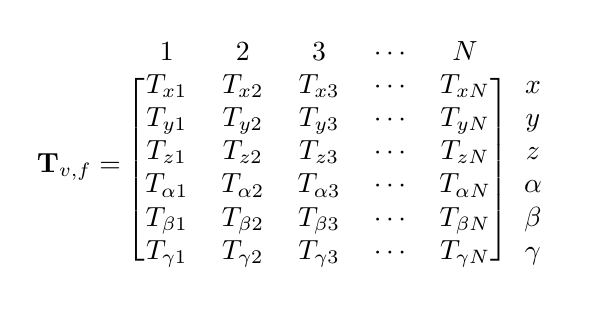
\begin{tikzpicture}
	\node [] {
		$
		 	\mathbf{T}_{v,f}= \begin{blockarray}{c c c c c c }
		 		1 & 2 & 3 & \cdots & N & \\
		 		\begin{block}{[c c c c c]c}
		 			T_{x1} & T_{x2} & T_{x3} & \cdots & T_{xN} & x\\
		 			T_{y1} & T_{y2} & T_{y3} & \cdots & T_{yN} & y\\
		 			T_{z1} & T_{z2} & T_{z3} & \cdots & T_{zN} & z\\
		 			T_{\alpha1} & T_{\alpha2} & T_{\alpha3} & \cdots & T_{\alpha N} & \alpha\\
		 			T_{\beta 1} & T_{\beta 2} & T_{\beta 3} & \cdots & T_{\beta N} & \beta\\
		 			T_{\gamma 1} & T_{\gamma 2} & T_{\gamma 3} & \cdots & T_{\gamma N} & \gamma \\
		 		\end{block}
		 	\end{blockarray}
		$
	};
	\end{tikzpicture}
\end{document}